\section{Αρχιτεκτονική υλοποίησης} \label{section:4-3-implementation-architecture}

Το σύστημα υλοποιήθηκε χρησιμοποιώντας το μοντέλο αρχιτεκτονικής των μικροϋπηρεσιών. Το μοντέλο των μικροϋπηρεσιών βασίζεται στην αποδόμηση του συστήματος σε μικρές μονάδες, οι οποίες συνεργάζονται ώστε να προσφέρουν ένα ενιαίο αποτέλεσμα. Η προσέγγιση αυτή έχει πολλά πλεονεκτήματα σε σύγκριση με την ανάπτυξη μονολιθικών εφαρμογών % todo: add reference
. Ο βασικός λόγος για τον οποίο επιλέχθηκε η αρχιτεκτονική μικροϋπηρεσιών είναι η ευκολία που προσφέρει στη γρήγορη ανάπτυξη καινούριων χαρακτηριστικών, ταυτόχρονα από διαφορετικά μέλη μίας ομάδας, ασύγχρονα και χωρίς την ανάγκη συνεχής επικοινωνίας και συνεννόησης μεταξύ τους. Αυτό συμβαίνει επειδή κάθε μέρος του συστήματος (υπηρεσία) είναι αυτόνομο και η ανάπτυξή του είναι διαχωρισμένη από το υπόλοιπο σύστημα με το οποίο είναι αδύναμα συνδεδεμένο (loosely coupled).

Το σύστημα συντίθεται από διάφορες μικροϋπηρεσίες, κάποιες από τις οποίες αναπτύχθηκαν στα πλαίσια αυτής της εργασίας ενώ άλλες αποτελούν δωρεάν λογισμικό ανοιχτού κώδικα. Οι μικροϋπηρεσίες αυτές συνοψίζονται στον παρακάτω πίνακα (πίνακας \ref{table:4-3-microservice-summary}).

\begin{table}[H]
    \begin{center}
        \begin{tabularx}{\textwidth}{l X}
            \toprule
            \textbf{Μικροϋπηρεσία} & \textbf{Σύντομη περιγραφή - Αντικείμενο/Στόχος} \\
            \midrule
            Concordia Application        & Υπηρεσία με την οποία αλληλεπιδρούν οι χρήστες. \\ [0.5ex]
            Concordia Contracts Migrator & Υπηρεσία μεταφόρτωσης των συμβολαίων (contracts) στο blockchain. \\ [0.5ex]
            Concordia Pinner             & Υπηρεσία καρφιτσώματος δεδομένων. \\ [0.5ex]
            Concordia Contracts Provider & Υπηρεσία διαμοιρασμού των contract artifacts μέσω HTTP. \\ [0.5ex]
            Ganache                      & Τοπικό, ιδιωτικό Ethereum blockchain. \\ [0.5ex]
            Rendezvous Server            & Υπηρεσία εύρεσης ομότιμων χρηστών. \\ [0.5ex]
            \bottomrule
        \end{tabularx}
    \end{center}
    \caption{Σύντομη περιγραφή υπηρεσιών συστήματος.}
    \label{table:4-3-microservice-summary}
\end{table}

Στα πλαίσια της εργασίας αναπτύχθηκαν επίσης διάφορα αρθρώματα, κυρίως με τη μορφή βιβλιοθηκών Javascript. Τα αρθρώματα χρησιμοποιούνται από τις υπηρεσίες για την επίτευξη των επιμέρους εργασιών. Η ανάπτυξη του λογισμικού σε ξεχωριστά αρθρώματα επιτρέπει την εύκολη επαναχρησιμοποίηση του κώδικα καθώς και τον διαχωρισμό των αυτόνομων τμημάτων κώδικα. Τα αρθρώματα συνοψίζονται στον παρακάτω πίνακα (πίνακας \ref{table:4-3-software-units-summary}).

\begin{table}[H]
    \begin{center}
        \begin{tabularx}{\textwidth}{l X}
            \toprule
            \textbf{Άρθρωμα} & \textbf{Σύντομη περιγραφή - Αντικείμενο/Στόχος} \\
            \midrule
            Άρθρωμα concordia-shared      & Χρήσιμα εργαλεία και σταθερές συστήματος. \\ [0.5ex]
            Άρθρωμα concordia-contracts   & Μεταγλώττιση των contracts και διάθεση των artifacts. \\ [0.5ex]
            Άρθρωμα eth-identity-provider & Δημιουργία μοναδικού αναγνωριστικού χρήστη για τη βάση OrbitDB. \\ [0.5ex]
            Άρθρωμα drizzle               & Βελτιωμένη προγραμματιστική διεπαφή επικοινωνίας με το blockchain. \\ [0.5ex]
            Άρθρωμα breeze                & Βελτιωμένη προγραμματιστική διεπαφή χρήσης της βάσης OrbitDB. \\ [0.5ex]
            \bottomrule
        \end{tabularx}
    \end{center}
    \caption{Σύντομη περιγραφή αρθρωμάτων συστήματος.}
    \label{table:4-3-software-units-summary}
\end{table}

Τα αρθρώματα και οι υπηρεσίες θα περιγραφούν σε μεγαλύτερη ανάλυση στα επόμενα κεφάλαια. Στο παρακάτω σχήμα (σχήμα \ref{figure:4-3-architecture-overview}) φαίνεται η συνολική αρχιτεκτονική του συστήματος.

\begin{figure}[H]
    \centering
    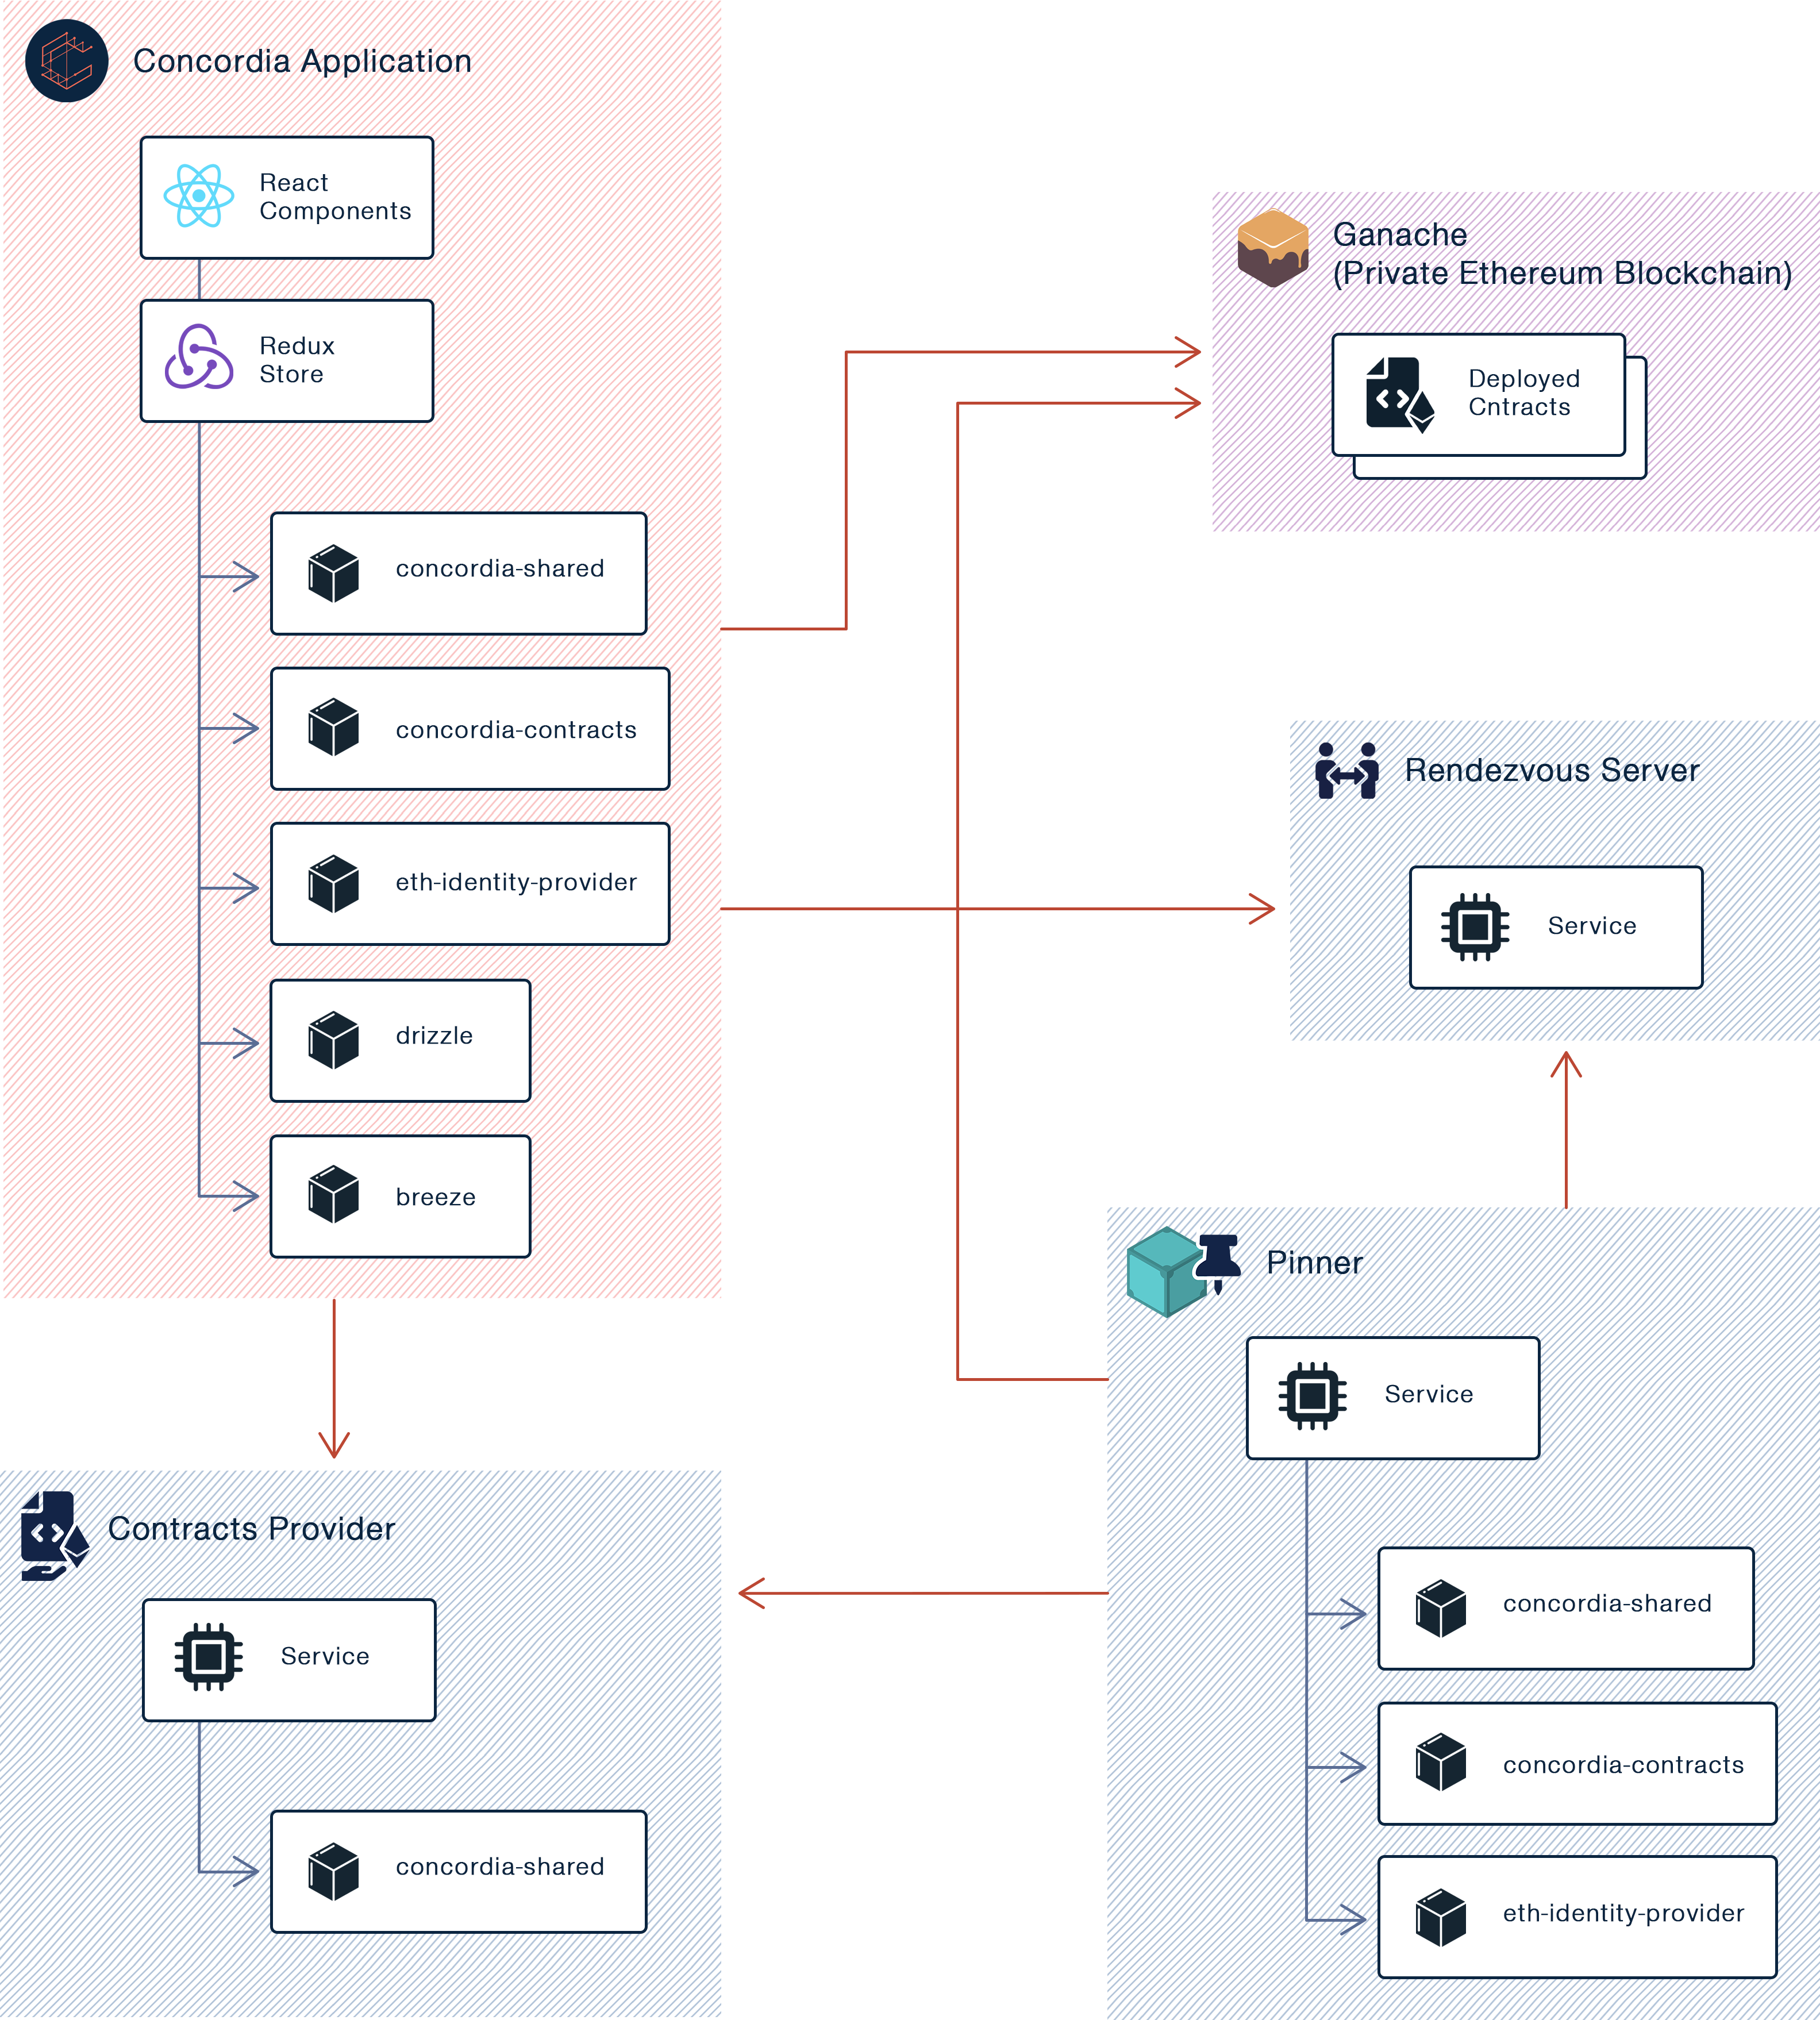
\includegraphics[width=.75\textwidth]{assets/figures/chapter-4/4.3.architecture-architecture-overview.png}
    \caption{Διάγραμμα αρχιτεκτονικής συστήματος}
    \label{figure:4-3-architecture-overview}
\end{figure}

% ===== =====
% Common software units
% ===== =====
\subsection{Αρθρώματα} \label{subsection:4-3-software-units}

Στο κεφάλαιο αυτό θα περιγραφούν με μεγαλύτερη λεπτομέρεια τα αρθρώματα που αναπτύχθηκαν.

\vspace{0.5cm}
\textbf{Άρθρωμα concordia-shared}

Το άρθρωμα concordia-shared αποτελεί μία βιβλιοθήκη χρήσιμων εργαλείων και σταθερών. Εδώ περιέχεται όλο το λογισμικό το οποίο πρέπει ή είναι επιθυμητό να συμπεριφέρεται με τον ίδιο τρόπο συνολικά στο σύστημα, όπως για παράδειγμα μέθοδοι παραμετροποίησης των υπηρεσιών και μέθοδοι καταγραφής (logging). Το άρθρωμα αυτό χρησιμοποιείται από το άρθρωμα concordia-contracts καθώς και από τις υπηρεσίες Concordia Application, Concordia Pinner και Concordia Contracts Provider.

% make more sense
Το άρθρωμα αυτό γίνεται διαθέσιμο για χρήση με τη μορφή τοπικής βιβλιοθήκης με τη χρήση της βιβλιοθήκης διαχείρισης μοναδικού αποθετηρίου κώδικα (monorepo) lerna.

\vspace{0.5cm}
\textbf{Άρθρωμα concordia-contracts}

Το άρθρωμα αυτό επιτελεί δύο ενέργειες. Αρχικά, είναι το άρθρωμα στο οποίο αναπτύσσονται τα contracts που χρησιμοποιούνται από την εφαρμογή. Το άρθρωμα αυτό αναλαμβάνει τη μεταγλώττιση των contracts από κώδικα γλώσσας Solidity, στην κατάλληλη τελική μορφή JSON. Παρέχονται επίσης σενάρια ενεργειών (scripts) ώστε τα contracts να μεταφορτωθούν σε blockchain καθώς και στην υπηρεσία Concordia Contracts Provider. Αποτελεί επίσης βιβλιοθήκη η οποία μετά τη μεταγλώττιση και μεταφόρτωση των contracts σε blockchain παρέχει τα contract artifacts. Χρησιμοποιείται από τις υπηρεσίες Concordia Application και Concordia Pinner.

Το άρθρωμα αυτό γίνεται διαθέσιμο για χρήση με τη μορφή τοπικής βιβλιοθήκης με τη χρήση της βιβλιοθήκης διαχείρισης monorepo lerna.

\vspace{0.5cm}
\textbf{Άρθρωμα eth-identity-provider}

Η λειτουργία της βάση OrbitDB απαιτεί τη δημιουργία ενός μοναδικού αναγνωριστικού χρήστη (identity). Για την εύκολη εξαγωγή ενός αναγνωριστικού χρήστη το οποίο να είναι μεν μοναδικό αλλά να είναι δυνατός ο επανυπολογισμός, χρησιμοποιήθηκε ο συνδυασμός της διεύθυνσης του χρήστη στο δίκτυο Ethereum με τη διεύθυνση του βασικού contract που χρησιμοποιεί η εφαρμογή. Ο υπολογισμός του συνδυασμού αυτού υλοποιείται από αυτό το άρθρωμα.

Το άρθρωμα αυτό γίνεται διαθέσιμο για χρήση με τη μορφή βιβλιοθήκης μέσω του αποθετηρίου λογισμικού npm.

\vspace{0.5cm}
\textbf{Άρθρωμα drizzle}

Το άρθρωμα drizzle που χρησιμοποιείται στην υπηρεσία Concordia Application είναι μία τροποποιημένη έκδοση της Javascript βιβλιοθήκης Drizzle που προσφέρεται από τη σουίτα εργαλείων Truffle. Η τροποποιημένη βιβλιοθήκη αναπτύχθηκε στα πλαίσια της διπλωματικής με στόχο τη διευκόλυνση της χρήσης του Drizle και την επιδιόρθωση προβληματικών σημείων της πρωτότυπης βιβλιοθήκης.

Το άρθρωμα drizzle υλοποιεί τις προγραμματιστικές διεπαφές μέσω των οποίων πραγματοποιείται η επικοινωνία της εφαρμογής με το blockchain. Για την επίτευξη της επικοινωνίας αυτής, η βιβλιοθήκη χρησιμοποιεί τη συλλογή βιβλιοθηκών web3.js η οποία αποτελεί τον πιο διαδεδομένο τρόπο διεπαφής με το blockchain σε αποκεντρωτικές εφαρμογές.

Το άρθρωμα αυτό γίνεται διαθέσιμο για χρήση με τη μορφή βιβλιοθήκης μέσω του αποθετηρίου λογισμικού npm.

\vspace{0.5cm}
\textbf{Άρθρωμα breeze}

Το άρθρωμα αυτό αποτελεί μία βιβλιοθήκη περίβλημα (wrapper) της βιβλιοθήκης OrbitDB. Η OrbitDB είναι μία βιβλιοθήκη η οποία προσφέρει τις απαραίτητες προγραμματιστικές διεπαφές για τη χρήση της βάσης δεδομένων με το ίδιο όνομα. Μέσα από τη χρήση των βιβλιοθηκών που προσφέρονται από το IPFS για την αποθήκευση δεδομένων, η OrbitDB καταφέρνει να υλοποιήσει μία αποκεντρωμένη βάση δεδομένων.

Το άρθρωμα breeze κάνει χρήση της βιβλιοθήκης OrbitDB, προσφέρει ωστόσο συγκεκριμένες προγραμματιστικές διεπαφές που διευκολύνουν τόσο την παραμετροποίηση της βάσης όσο και τη χρήση της, ενώ όπως και στο άρθρωμα drizzle το άρθρωμα breeze αναλαμβάνει να διορθώσει ορισμένα προβλήματα της πρωτότυπης βιβλιοθήκης.

Το άρθρωμα αυτό γίνεται διαθέσιμο για χρήση με τη μορφή βιβλιοθήκης μέσω του αποθετηρίου λογισμικού npm.

% ===== =====
% concordia-app microservice
% ===== =====
\subsection{Concordia Application} \label{subsection:4-3-concordia-application-service}

\vspace{0.5cm}
\textbf{Περιγραφή - Στόχοι υπηρεσίας}

Η εφαρμογή Concordia (Concordia Application) εκθέτει τις γραφικές διεπαφές μέσω των οποίων αλληλεπιδρούν οι χρήστες με το σύστημα. Αποτελεί τον δίαυλο επικοινωνίας του τελικού χρήστη με το blockchain και με τη βάση OrbitDB. Η αρχιτεκτονική της υπηρεσίας φαίνεται στο σχήμα \ref{figure:4-3-concordia-application-architecture}. Μέσω της εφαρμογής Concordia οι χρήστες μπορούν να:

\begin{itemize}
    \item περιηγηθούν και διαβάσουν το περιεχόμενο της πλατφόρμας

    \item δημιουργήσουν λογαριασμό χρήστη

    \item δημοσιεύσουν και τροποποιήσουν προσωπικές τους πληροφορίες όπως η τοποθεσία και η εικόνα προφίλ

    \item δημιουργήσουν θέματα (topics)

    \item δημιουργήσουν ψηφοφορίες (polls), καθώς και να ψηφίσουν σε αυτές

    \item δημιουργήσουν και τροποποιήσουν μηνύματα (posts)

    \item υπερψηφίσουν (up-vote) ή καταψηφίσουν (down-vote) μηνύματα άλλων χρηστών
\end{itemize}

Η υπηρεσία αποτελείται από κώδικα γραμμένο σε Javascript ο οποίος γίνεται διαθέσιμος στους τελικούς χρήστες με τη μορφή εφαρμογής διαδικτύου (web application) μέσω ενός διακομιστή (server). Παρόλο που η υπηρεσία προσφέρει τη γραφική διεπαφή χρήστη μόνο στην αγγλική γλώσσα, έχει παραμετροποιηθεί ώστε να είναι δυνατή η εύκολη μεταγλώττιση της χωρίς την ανάγκη πραγματοποίησης μεγάλων αλλαγών στον κώδικα.

Χρησιμοποιείται η βιβλιοθήκη React για την οργάνωση και ανάπτυξη των συνθετικών τμημάτων (components) του γραφικού περιβάλλοντος. Για το γραφικό περιβάλλον γίνεται χρήση του framework της Semantic UI. Χρησιμοποιείται η βιβλιοθήκη Redux για τη διαχείριση κατάστασης της εφαρμογής (state management), % todo: find a better greek translation
καθώς και η βιβλιοθήκη Redux-Saga για τη διαχείριση ασύγχρονων παράπλευρων ενεργειών (side-effects) σε ένα σύστημα βασισμένο σε συμβάντα (event-based). Άλλες βιβλιοθήκες χρησιμοποιούνται για διάφορα μέρη της υπηρεσίας, ενώ χρησιμοποιούνται επίσης τα αρθρώματα που περιγράφηκαν προηγουμένως για την επίτευξη διαφορετικών στόχων. Ο πλήρης κατάλογος των βιβλιοθηκών και αρθρωμάτων μπορεί να βρεθεί στον κώδικα της υπηρεσίας στο παράρτημα. % todo: add reference to the appendix containing the code or a link to it in the repo

\begin{figure}[H]
    \centering
    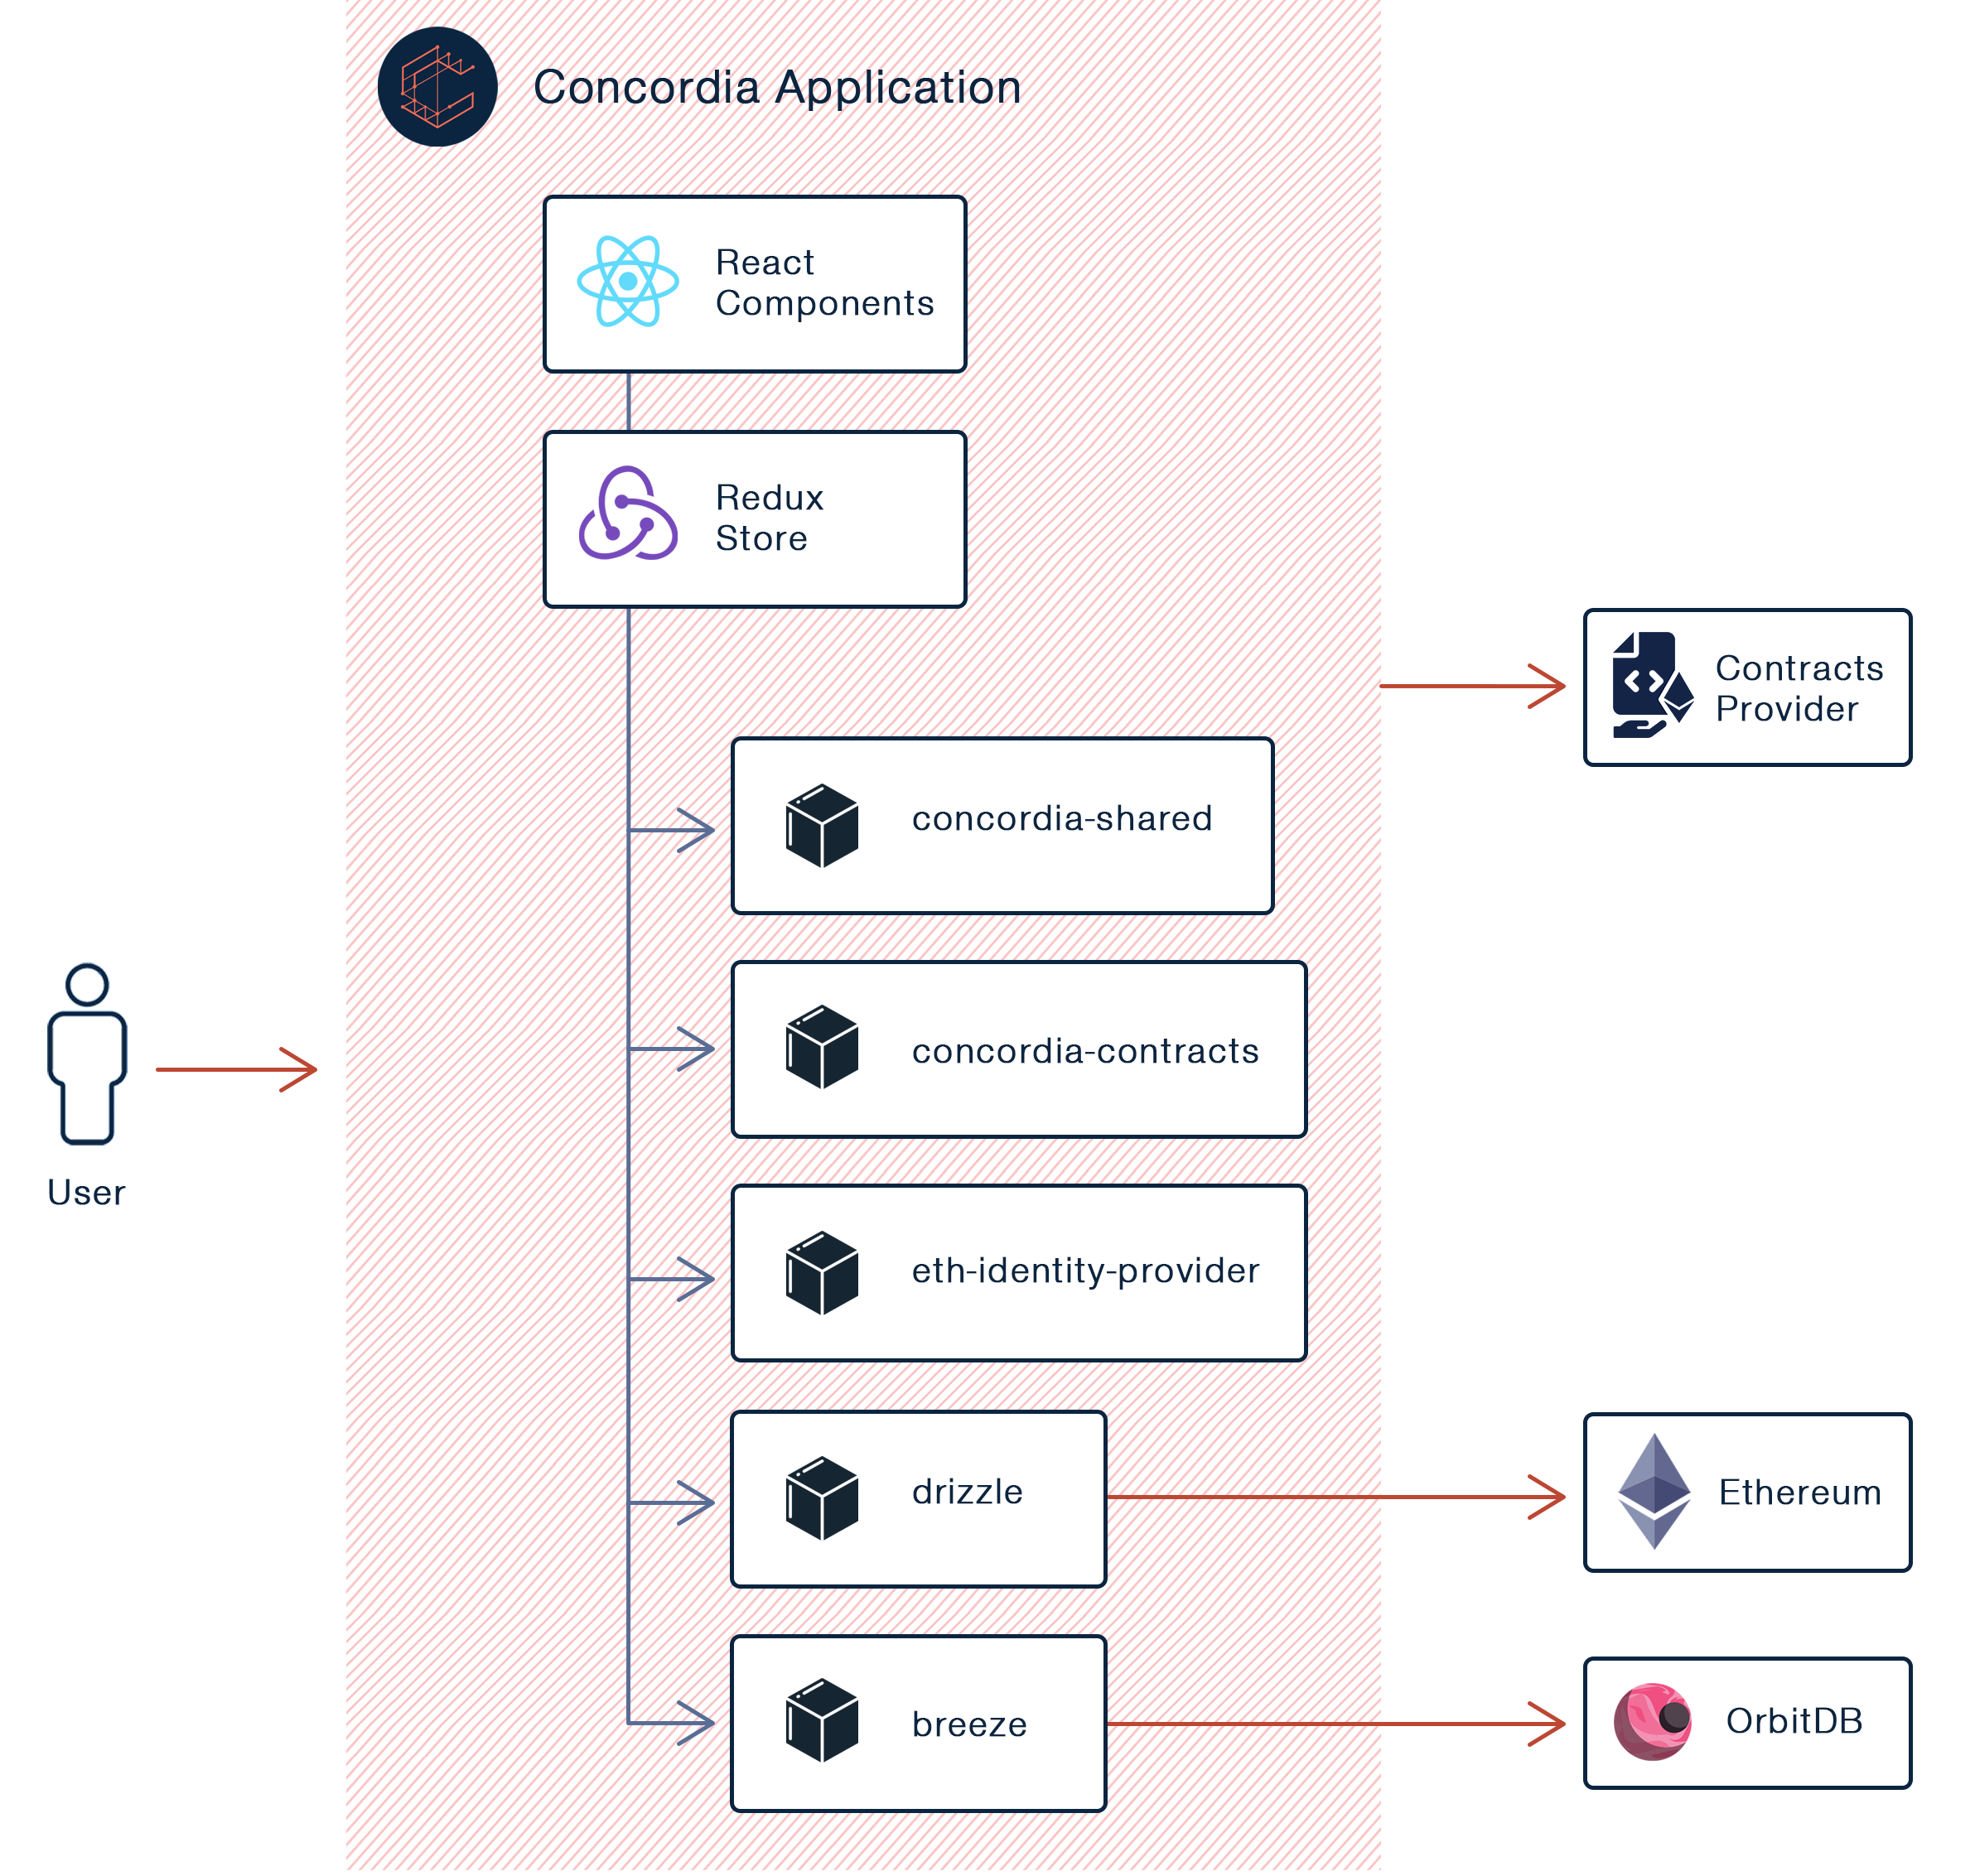
\includegraphics[width=.7\textwidth]{assets/figures/chapter-4/4.3.architecture-4.3.2.concordia-application-architecture.png}
    \caption{Αρχιτεκτονική υπηρεσίας Concordia Application}
    \label{figure:4-3-concordia-application-architecture}
\end{figure}

Για τη λειτουργία της υπηρεσία Concordia Application είναι απαραίτητα τα αντικείμενα (artifacts) που προκύπτουν από τη μεταγλώττιση των contracts και τη μεταφόρτωση/δημοσίευσή τους στο blockchain. Για την εισαγωγή των artifacts στην υπηρεσία έχουν αναπτυχθεί δύο μέθοδοι.

Η πρώτη μέθοδος είναι η μεταγλώττιση και μεταφόρτωση των contracts πριν την παραγωγή του πακέτου λογισμικού της υπηρεσίας για τελική χρήση (production build). Με αυτό τον τρόπο η υπηρεσία θα έχει πρόσβαση στα artifacts μέσω της βιβλιοθήκης που παράγεται από το άρθρωμα concordia-contracts. Αυτή η μέθοδος έχει το μειονέκτημα ότι το τελικό πακέτο λογισμικού (production build) ``δένεται'' με όποια συγκεκριμένη έκδοση των contracts είναι διαθέσιμη κατά τη δημιουργία του πακέτου. Αυτό σημαίνει ότι σε ενδεχόμενη ενημέρωση των contracts πρέπει αναγκαστικά να δημιουργηθεί και νέα έκδοση του πακέτου λογισμικού της υπηρεσίας Concordia Application.

Για την αποφυγή του παραπάνω προβλήματος αναπτύχθηκε η δεύτερη μέθοδος προσκόμισης των contract artifacts, η οποία είναι η λήψη τους (download) από μία άλλη τοποθεσία στο διαδίκτυο. Σε αυτή τη μέθοδο, η εφαρμογή κατά την εκκίνησή της πραγματοποιεί ένα HTTP αίτημα (HTTP request) σε διεύθυνση η οποία δίνεται ως μεταβλητή περιβάλλοντος (environment variable). Η απάντηση του αιτήματος αναμένεται να περιέχει τα artifacts ώστε η εφαρμογή να τα χρησιμοποιήσει.

\vspace{0.5cm}
\textbf{Διανομή}

Η υπηρεσία Concordia Application πακετάρεται μαζί με τον διακομιστή nginx και γίνεται διαθέσιμη για χρήση ως εικόνα docker (docker image) μέσω του αποθετηρίου εικόνων dockerhub. Κατά την εκτέλεση της εικόνας οι χρήστες μπορούν μέσω μεταβλητών περιβάλλοντος να ορίσουν παραμέτρους της εκτέλεσης όπως η διεύθυνση του εξυπηρετητή (host location) της εφαρμογής και οι τοποθεσίες των υπηρεσιών Rendezvous Server και Contracts Provider.

% ===== =====
% concordia-contracts-migrator microservice
% ===== =====
\subsection{Concordia Contracts Migrator} \label{subsection:4-3-concordia-contracts-migrator}

\vspace{0.5cm}
\textbf{Περιγραφή - Στόχοι υπηρεσίας}

Η υπηρεσία αυτή αποτελείται από ένα εκτελέσιμο πρόγραμμα γραμμής εντολών βασισμένο στο άρθρωμα concordia-contracts που αναλύθηκε σε προηγούμενη υποενότητα (\ref{subsection:4-3-software-units}). Το πρόγραμμα, κατά την εκτέλεσή του, μεταγλωττίζει τα contracts και έπειτα τα μεταφορτώνει στο blockchain το οποίο είναι ορισμένο με χρήση μεταβλητών περιβάλλοντος. Τέλος, αν οι κατάλληλες μεταβλητές περιβάλλοντος είναι ορισμένες, το πρόγραμμα μεταφορτώνει τα τελικά artifacts σε αποθετήριο Concordia Contracts Provider. Η αρχιτεκτονική της υπηρεσίας φαίνεται στο παρακάτω σχήμα (σχήμα \ref{figure:4-3-concordia-contracts-migrator-architecture}).

\begin{figure}[H]
    \centering
    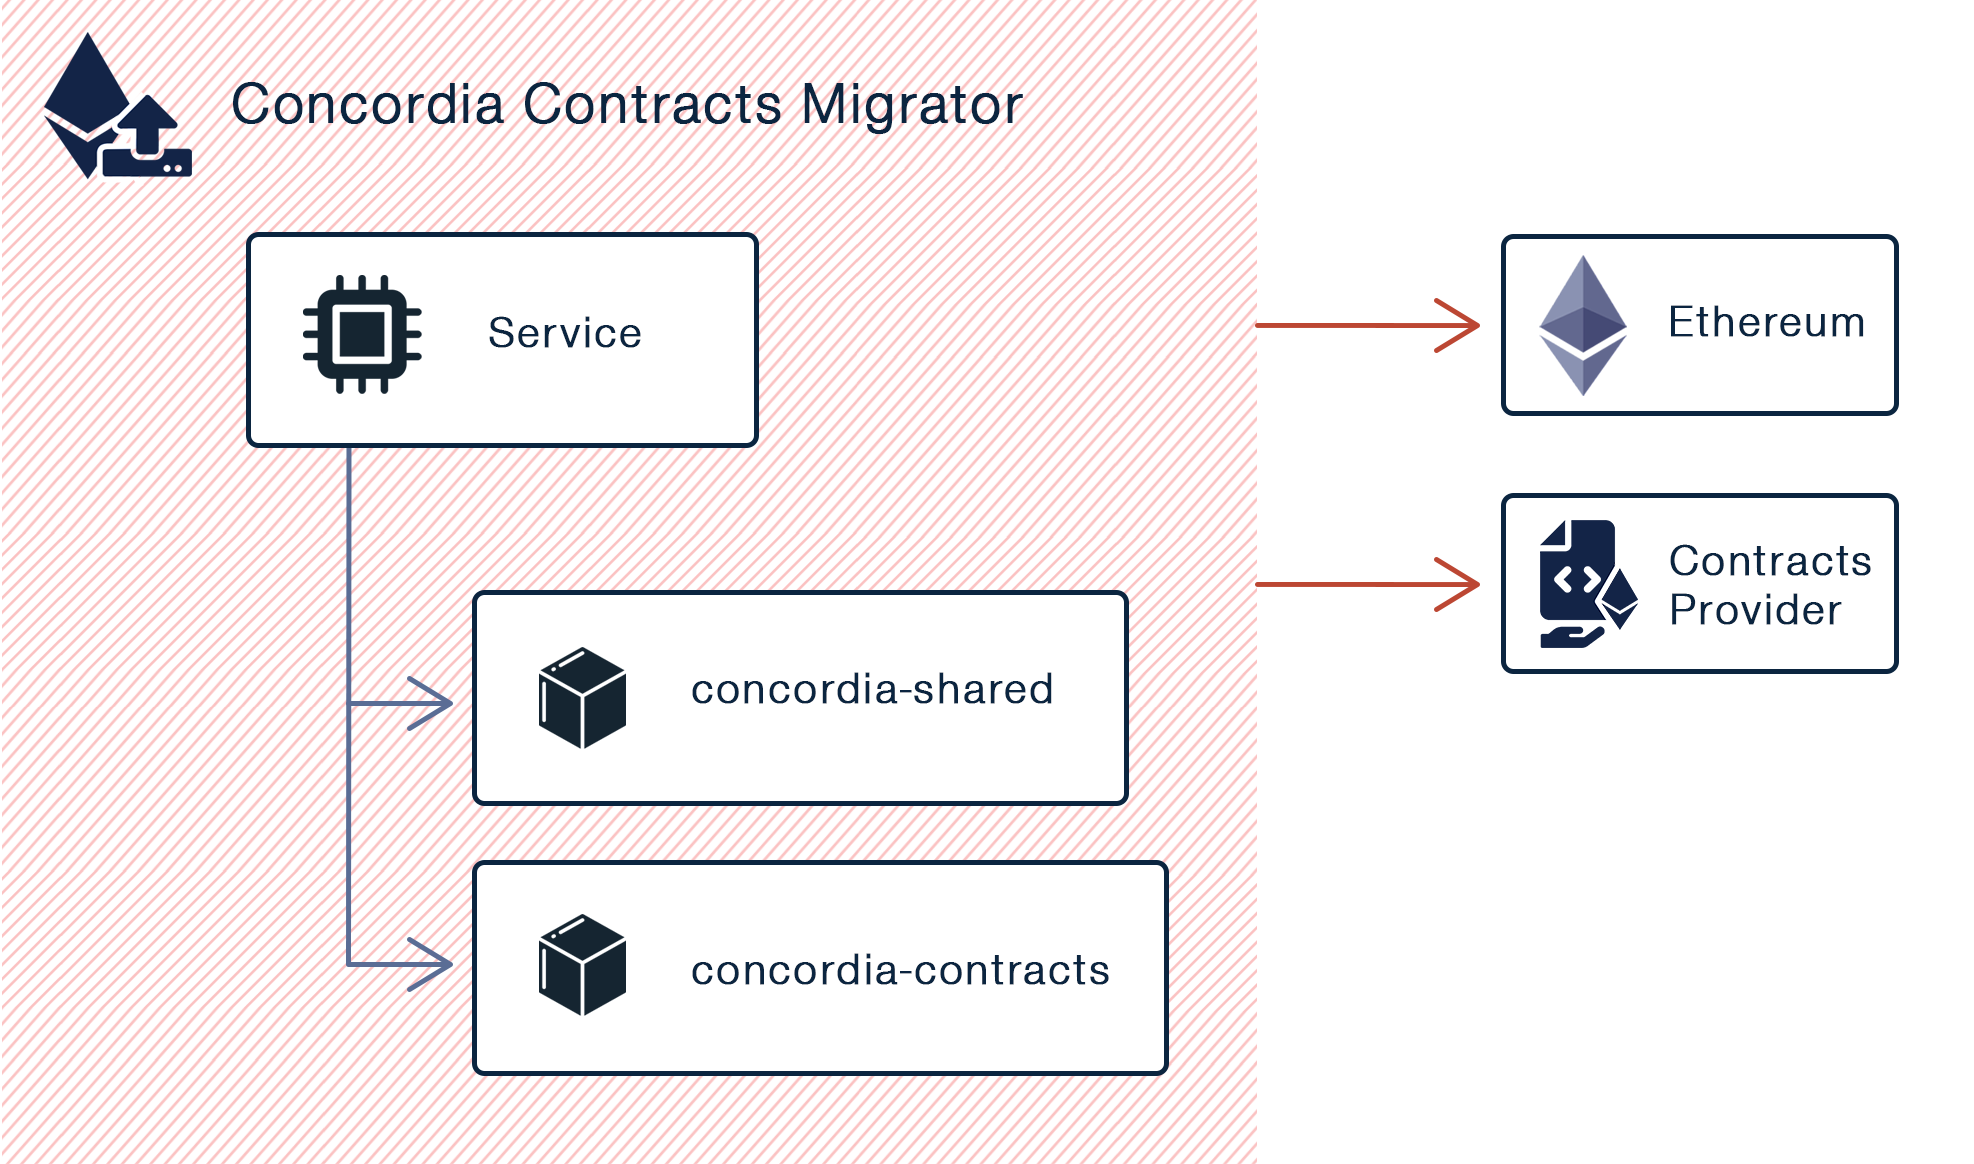
\includegraphics[width=.6\textwidth]{assets/figures/chapter-4/4.3.architecture-4.3.3.concordia-contracts-migrator-architecture.png}
    \caption{Αρχιτεκτονική υπηρεσίας Concordia Contracts Migrator}
    \label{figure:4-3-concordia-contracts-migrator-architecture}
\end{figure}

\vspace{0.5cm}
\textbf{Διανομή}

Η υπηρεσία αυτή γίνεται διαθέσιμη για χρήση ως docker image μέσω του αποθετηρίου εικόνων dockerhub. Οι χρήστες μπορούν χρησιμοποιώντας μεταβλητές περιβάλλοντος να αλλάξουν τη διεύθυνση του blockchain και την τοποθεσία της υπηρεσίας Contracts Provider στην οποία το πρόγραμμα θα μεταφορτώσει τα contracts και τα artifacts.

% ===== =====
% concordia-pinner microservice
% ===== =====
\subsection{Concordia Pinner} \label{subsection:4-3-concordia-pinner-service}

\vspace{0.5cm}
\textbf{Περιγραφή - Στόχοι υπηρεσίας}

Η υπηρεσία καρφιτσώματος περιεχομένου (Concordia Pinner) αποτελεί μία εφαρμογή τερματικού (temrinal application/cmd application) η οποία στοχεύει στο καρφίτσωμα (pinning) του περιεχομένου που αποθηκεύεται στο IPFS μέσω της βάσης OrbitDB. Η υπηρεσία είναι γραμμένη στη γλώσσα προγραμματισμού Javascript. Η αρχιτεκτονική της υπηρεσίας φαίνεται το σχήμα \ref{figure:4-3-concordia-pinner-architecture}.

\begin{figure}[H]
    \centering
    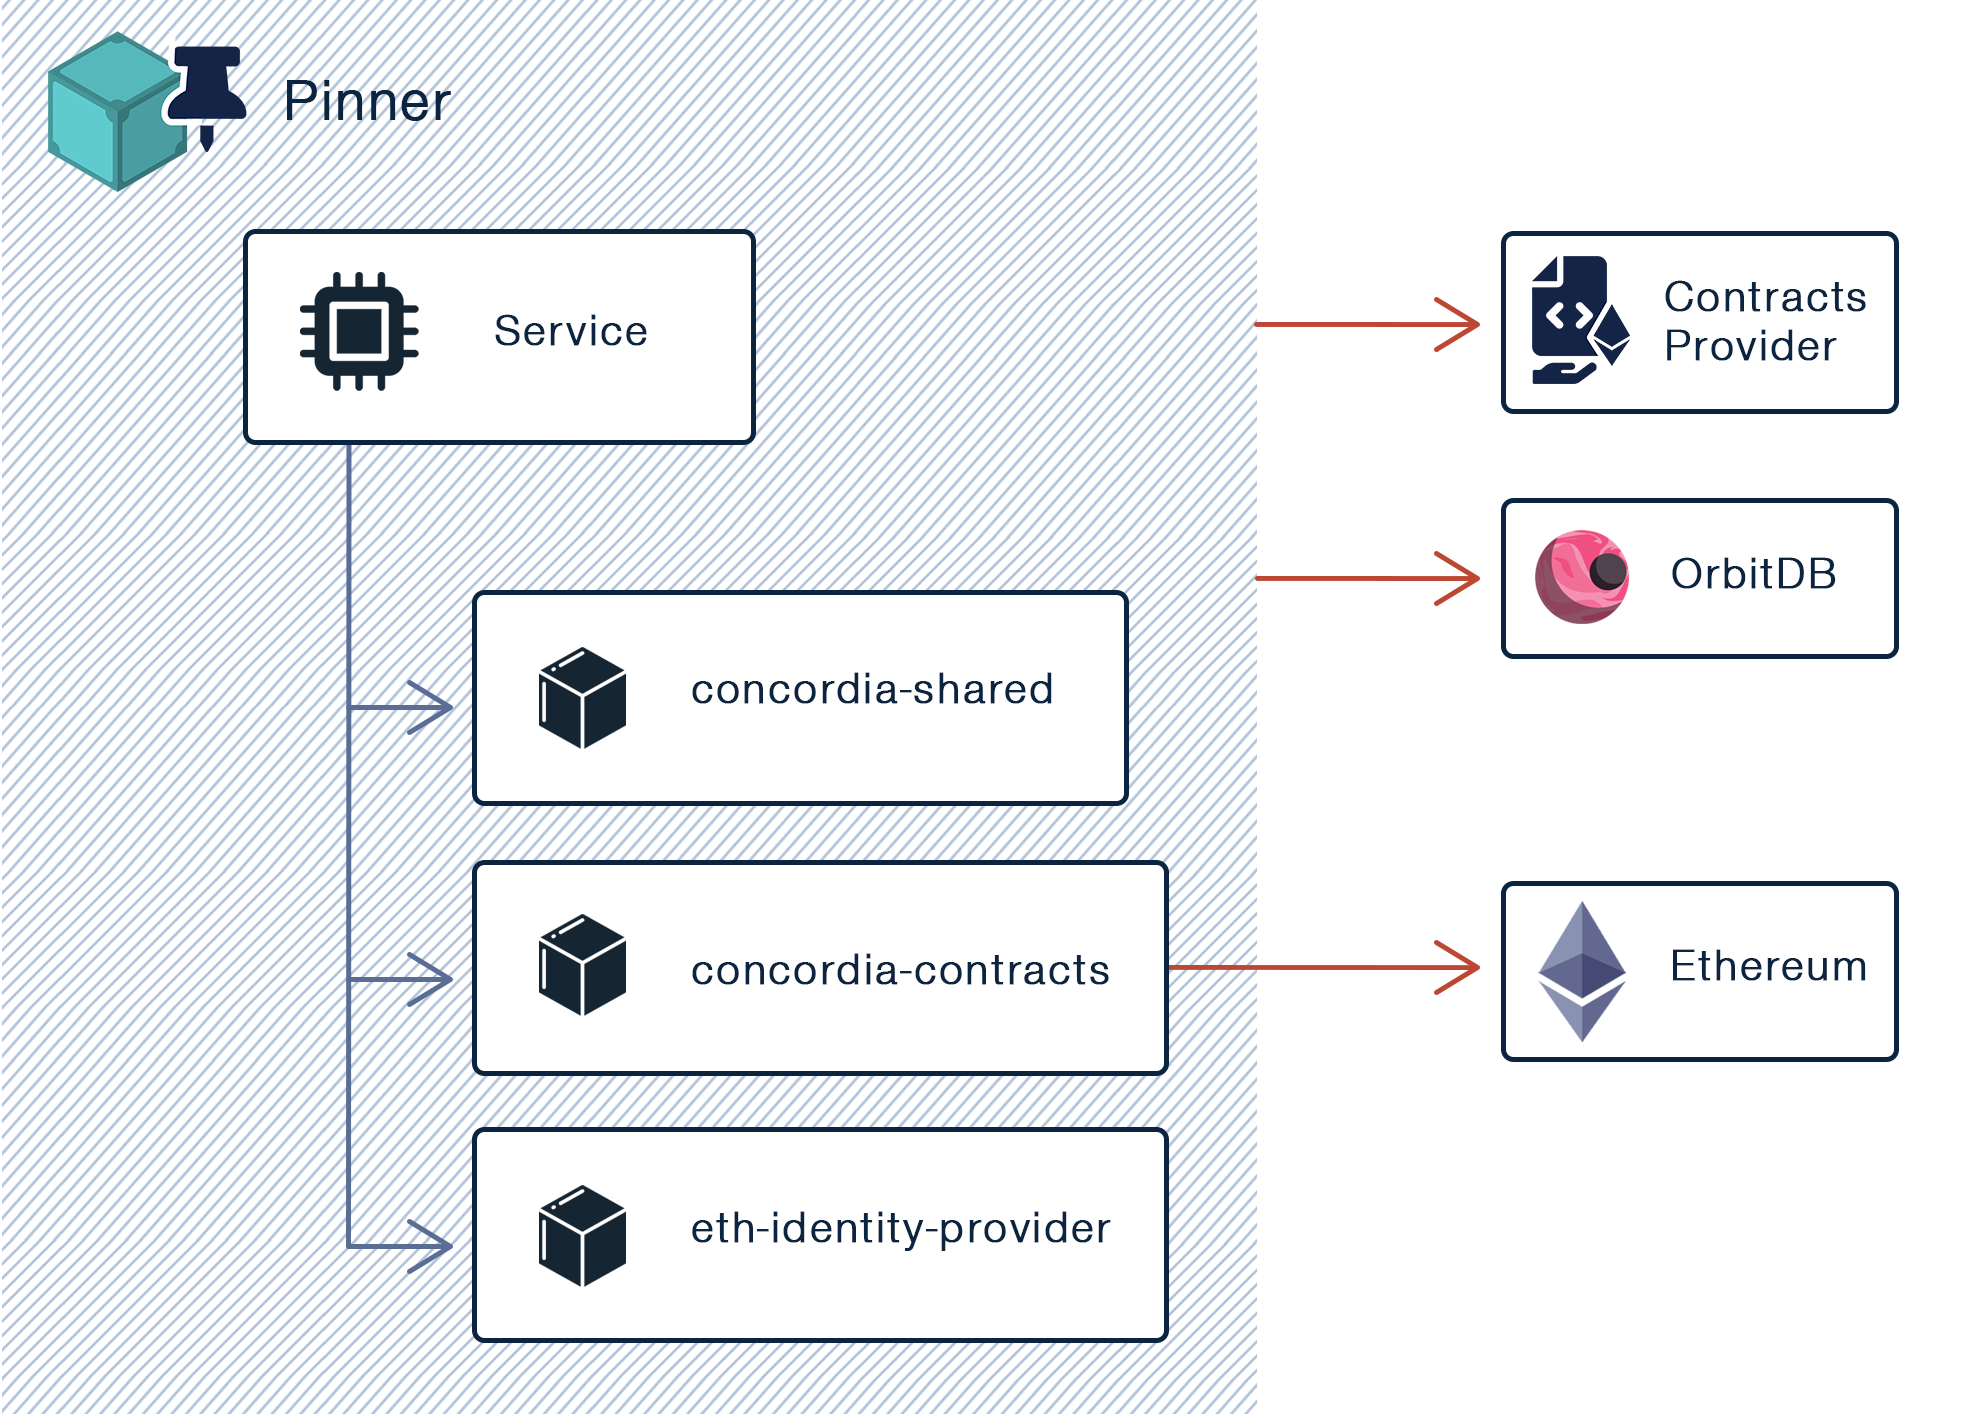
\includegraphics[width=.6\textwidth]{assets/figures/chapter-4/4.3.architecture-4.3.4.concordia-pinner-architecture.png}
    \caption{Αρχιτεκτονική υπηρεσίας Concordia Pinner}
    \label{figure:4-3-concordia-pinner-architecture}
\end{figure}

Η υπηρεσία αυτή υλοποιήθηκε για να εγγυηθεί η διαθεσιμότητα του περιεχομένου του συστήματος που αποθηκεύεται στο IPFS (τίτλοι θεμάτων, περιεχόμενο μηνυμάτων και άλλα). Λόγω του τρόπου λειτουργίας % todo: insert reference
του IPFS, το περιεχόμενο που αναρτούν οι χρήστες πρέπει να καρφιτσώνεται από άλλους χρήστες ή αυτόνομες εφαρμογές, όπως η υπηρεσία Concordia Pinner, ώστε να είναι διαθέσιμο. Αν το περιεχόμενο δεν καρφιτσωθεί, τότε θα είναι διαθέσιμο στους υπόλοιπους χρήστες μόνο από %todo: fix gender stuff
τον/τη δημιουργό, έτσι αν αυτός/αυτή δεν είναι ενεργός/ενεργή στο δίκτυο, το περιεχόμενο θα είναι αδύνατο να βρεθεί.

Η υπηρεσία συνδέεται στο blockchain από όπου παρακολουθεί την κατάσταση του συστήματος και ``ακούει'' για νέους χρήστες, θέματα και μηνύματα. Η υπηρεσία συνδέεται επίσης στο IPFS, έτσι όταν δημιουργηθεί νέο περιεχόμενο στο σύστημα το καρφιτσώνει αυτόματα. Με αυτό τον τρόπο, διατηρώντας την υπηρεσία πάντα διαθέσιμη, για παράδειγμα εκτελώντας τη σε περιβάλλον διακομιστή (server), διαβεβαιώνεται η διαθεσιμότητα του περιεχομένου.

\vspace{0.5cm}
\textbf{Διανομή}

Η υπηρεσία αυτή γίνεται διαθέσιμη για χρήση ως docker image μέσω του αποθετηρίου εικόνων dockerhub. Κατά την εκτέλεση της εικόνας οι χρήστες μπορούν μέσω μεταβλητών περιβάλλοντος να ορίσουν παραμέτρους της υπηρεσίας όπως τη διεύθυνση του εξυπηρετητή (host location), τη διεύθυνση του blockchain, τις διαδρομές αποθήκευσης των δεδομένων στο σύστημα και τις τοποθεσίες των υπηρεσιών Rendezvous Server και Contracts Provider.

% ===== =====
% concordia-contracts-provider microservice
% ===== =====
\subsection{Concordia Contracts Provider} \label{subsection:4-3-concordia-contracts-provider-service}

\vspace{0.5cm}
\textbf{Περιγραφή - Στόχοι υπηρεσίας}

Η υπηρεσία Contracts Provider αποτελεί μία βοηθητική υπηρεσία η οποία υλοποιεί ένα απλό αποθετήριο για τα contract artifacts. Είναι γραμμένη σε Javascript και διαθέτει δύο HTTP \textenglish{endpoints}, ένα για τη μεταφόρτωση (upload) των artifacts προς την υπηρεσία και ένα για τη λήψη (download) από την υπηρεσία. Η υπηρεσία υποστηρίζει επίσης την επισύναψη ετικετών στα artifacts, όπως η έκδοση (version) ή το κλαδί ανάπτυξης (branch, για παράδειγμα \textenglish{master/develop}). Η αρχιτεκτονική της υπηρεσίας φαίνεται το σχήμα \ref{figure:4-3-concordia-contracts-provider-architecture}.

\begin{figure}[H]
    \centering
    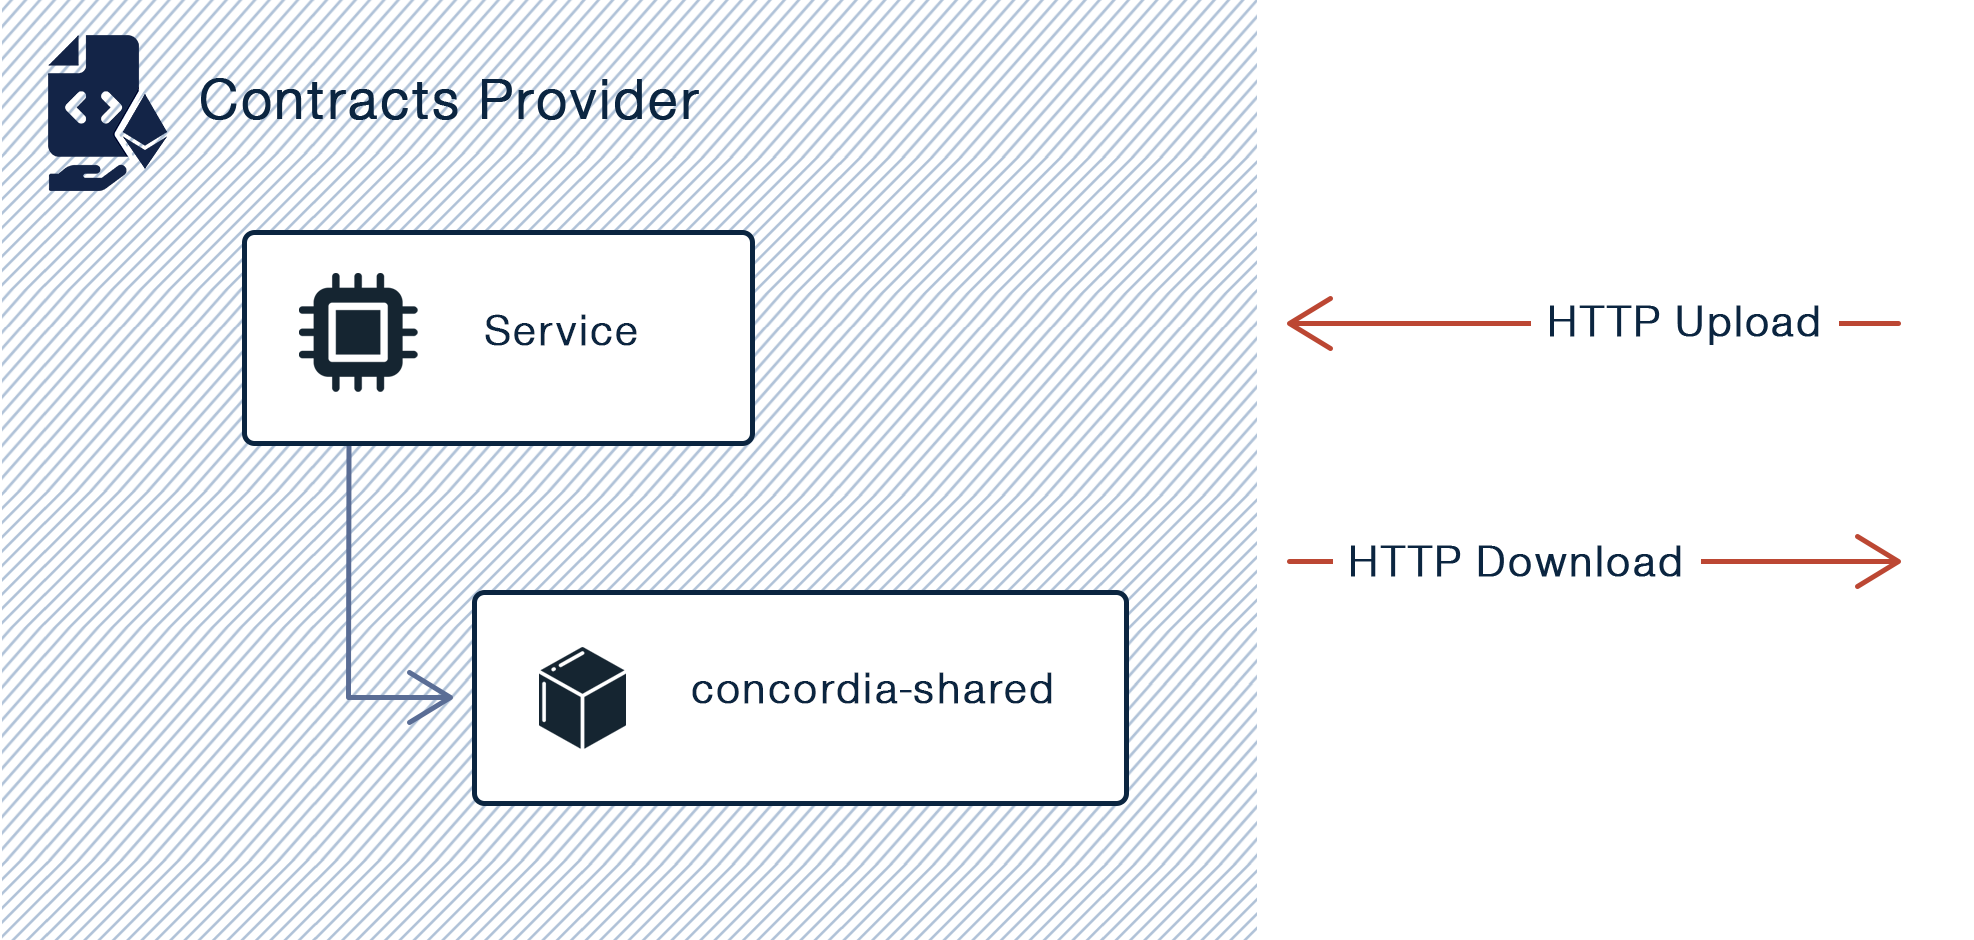
\includegraphics[width=.6\textwidth]{assets/figures/chapter-4/4.3.architecture-4.3.5.concordia-contracts-provider-architecture.png}
    \caption{Αρχιτεκτονική υπηρεσίας Concordia Contracts Provider}
    \label{figure:4-3-concordia-contracts-provider-architecture}
\end{figure}

Η υπηρεσία χρησιμοποιείται σε μία προσπάθεια αποσύνδεσης της βασικής εφαρμογής που υλοποιεί η υπηρεσία Concordia Application από μία συγκεκριμένη έκδοση των contracts. Οι λόγοι που αυτό είναι επιθυμητό αναπτύχθηκαν στην περιγραφή της υπηρεσίας Concordia \textenglish{Application} (υποενότητα \ref{subsection:4-3-concordia-application-service}). Ωστόσο, η υπηρεσία Contracts Provider αποτελεί σημείο κεντροποίησης του συστήματος, για το λόγο αυτό θεωρείται προσωρινή λύση η οποία θα μπορούσε να αντικατασταθεί από αποκεντρωτικές λύσεις όπως η μεταφόρτωση των artifacts στο IPFS και ο διαμοιρασμός τους από εκεί.

\vspace{0.5cm}
\textbf{Διανομή}

Η υπηρεσία αυτή γίνεται διαθέσιμη για χρήση ως docker image μέσω του αποθετηρίου εικόνων dockerhub. Οι χρήστες μπορούν χρησιμοποιώντας μεταβλητές περιβάλλοντος να αλλάξουν παραμέτρους της εκτέλεσης όπως η διαδρομή αποθήκευσης των μεταφορτωμένων contract artifacts.

% ===== =====
% rendezvous-ganache microservice
% ===== =====
\subsection{Ganache} \label{subsection:4-3-ganache-service}

\vspace{0.5cm}
\textbf{Περιγραφή - Στόχοι υπηρεσίας}

Η υπηρεσία Ganache αποτελεί μία εφαρμογή τερματικού η οποία είναι μέρος της δωρεάν σουίτας ανοιχτού λογισμικού Truffle. Η εφαρμογή δημιουργεί ένα τοπικό, ιδιωτικό blockchain το οποίο ακολουθεί το πρότυπο του Ethereum. Επίσης, η εφαρμογή δρα ως minner στο δίκτυο, διεκπεραιώνοντας όλες τις συναλλαγές.

\vspace{0.5cm}
\textbf{Διανομή}

Για τη χρήση της υπηρεσίας αυτής αναπτύχθηκε μία νέα εικόνα docker που βασίζεται στην επίσημη εικόνα που διατίθεται από τη σουίτα και προσθέτει μερικές χρήσιμες λειτουργικότητες όπως η δυνατότητα αποκάλυψης των κλειδιών που δημιουργούνται κατά την εκτέλεση. Η υπηρεσία γίνεται διαθέσιμη για χρήση ως docker image μέσω του αποθετηρίου εικόνων dockerhub. Η εικόνα παρέχει τη δυνατότητα τροποποίησης των παραμέτρων εκτέλεσης με χρήση μεταβλητών περιβάλλοντος. Με αυτό τον τρόπο οι χρήστες μπορούν να αλλάξουν τον αριθμό των λογαριασμών που θα δημιουργηθούν, το ποσό του Ether που θα λάβει κάθε λογαριασμός καθώς και άλλες μεταβλητές.

% ===== =====
% rendezvous-server microservice
% ===== =====
\subsection{Rendezvous Server} \label{subsection:4-3-rendezvous-server-service}

\vspace{0.5cm}
\textbf{Περιγραφή - Στόχοι υπηρεσίας}

Η υπηρεσία Rendezvous Server αποτελεί δωρεάν λογισμικό ανοιχτού κώδικα το οποίο χρησιμοποιήθηκε (αλλά δεν αναπτύχθηκε) στα πλαίσια της διπλωματικής και υλοποιεί το πρωτόκολλο rendezvous για την εύρεση ομότιμων χρηστών (peers). Η υπηρεσία είναι απαραίτητη για τη λειτουργία του IPFS, ώστε οι ομότιμοι χρήστες (peers) να μπορούν να ανακαλύψουν τις διευθύνσεις των υπόλοιπων χρηστών του δικτύου.

\vspace{0.5cm}
\textbf{Διανομή}

Η υπηρεσία αυτή είναι διαθέσιμη για χρήση από τους δημιουργούς της τόσο ως εφαρμογή μέσω του αποθετηρίου λογισμικού npm αλλά και ως docker image μέσω του αποθετηρίου εικόνων dockerhub.

% ===== =====
% microservice communication
% ===== =====
\subsection{Διασύνδεση υπηρεσιών} \label{subsection:4-3-service-communication}

Στο μοντέλο των μικροϋπηρεσιών, βασικό χαρακτηριστικό είναι η επικοινωνία των ξεχωριστών υπηρεσιών και η ανταλλαγή μηνυμάτων για την επίτευξη των λειτουργικοτήτων του συστήματος. Σε αυτήν την υποενότητα θα αναλυθεί ο τρόπος με τον οποίο οι μικροϋπηρεσίες επικοινωνούν μεταξύ τους καθώς και η φύση και το περιεχόμενο των μηνυμάτων που ανταλλάσουν.

Στο παρακάτω σχήμα (σχήμα \ref{figure:4-3-communications-graph}) φαίνεται ο γράφος που οπτικοποιεί τα κανάλια επικοινωνίας μεταξύ των μικροϋπηρεσιών, καθώς και τα κανάλια επικοινωνίας των μικροϋπηρεσιών με το blockchain.

\begin{figure}[H]
    \centering
    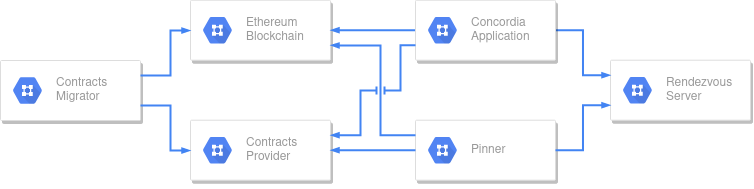
\includegraphics[width=.9\textwidth]{assets/figures/chapter-4/4.3.communications-diagram.png}
    \caption{Γράφος οπτικοποίησης των καναλιών επικοινωνίας των μικροϋπηρεσιών}
    \label{figure:4-3-communications-graph}
\end{figure}

Εδώ αναλύεται η επικοινωνία κάθε μικροϋπηρεσίας:

\begin{itemize}
    \item \textbf{Contracts Migrator}: η υπηρεσία εκτελεί αίτημα HTTP κατά την μεταφόρτωση των \textenglish{contracts} στο Ethereum blockchain, επίσης εκτελεί αίτημα HTTP για την μεταφόρτωση των contract artifacts στην υπηρεσία Contracts Provider

    \item \textbf{Concordia Application}: η υπηρεσία εκτελεί αίτημα HTTP για την λήψη των contract \textenglish{artifacts} από την υπηρεσία Contracts Provider, εκτελεί αιτήματα HTTP για την διενέργεια συναλλαγών στο Ethereum blockchain και τέλος δημιουργεί κανάλι UDP επικοινωνίας με την υπηρεσία Rendezvous Server για την ανακάλυψη ομότιμων χρηστών (peers) στο δίκτυο IPFS

    \item \textbf{Pinner}: η υπηρεσία εκτελεί αίτημα HTTP για την λήψη των contract artifacts από την υπηρεσία Contracts Provider, εκτελεί αιτήματα HTTP για την ανανέωση και παρατήρηση της κατάστασης του contract στο Ethereum blockchain και τέλος δημιουργεί κανάλι UDP επικοινωνίας με την υπηρεσία Rendezvous Server για την ανακάλυψη peers στο δίκτυο IPFS

    \item \textbf{Rendezvous Server}: η υπηρεσία διατηρεί ανοιχτά κανάλια UDP επικοινωνίας με τους ομότιμους χρήστες μέσω των οποίων ενημερώνει την λίστα των διαθέσιμων, ενεργών χρηστών

    \item \textbf{Contracts Provider}: η υπηρεσία δεν υποκινεί καμία επικοινωνία παρά μόνο απαντά σε αιτήματα επικοινωνία από άλλες υπηρεσίες
\end{itemize}

% ===== =====
% data flow
% ===== =====
\subsection{Ροή πληροφορίας} \label{subsection:4-3-data-flow}

Στην παρούσα υποενότητα θα αναλυθεί η ροή της πληροφορίας στο σύστημα. Λόγω των πολλαπλών υπηρεσιών, της κατάτμησης την πληροφορίας και των διαφορετικών σημείων αποθήκευσης της, η ροή της πληροφορίας στο σύστημα ακολουθεί ένα σχετικά περίπλοκο μονοπάτι (σε σχέση με κλασσικές, μονολιθικές, κεντροποιημένες εφαρμογές).

Αρχικά θα γίνει αναφορά στη διαδικασία αποθήκευσης των νέων πληροφοριών. Η μοναδική πηγή παραγωγής δεδομένων στο σύστημα είναι οι χρήστες και κατ' επέκταση η υπηρεσία Concordia Application, εφόσον είναι η μοναδική υπηρεσία με την οποία αυτοί αλληλεπιδρούν. Τα δεδομένα που δημιουργούν οι χρήστες (πληροφορίες χρηστών, τίτλοι θεμάτων και περιεχόμενο μηνυμάτων) κατατμήζονται πριν αποθηκευτούν. Η πληροφορία που εισάγεται στο σύστημα κατατμήζεται σε δύο μέρη. Στο blockchain αποθηκεύεται ένας δείκτης προς τα δεδομένα, ενώ τα πραγματικά δεδομένα αποθηκεύονται στη βάση OrbitDB. Ο δείκτης εκτός από την άμεση χρησιμότητα στην εύρεση των δεδομένων, παρέχει και την έμμεση λειτουργικότητα της δημιουργίας απαραίτητων μεταδομένων όπως ο αριθμός των θεμάτων στο σύστημα ή των μηνυμάτων σε ένα θέμα.

Από την πλευρά της εύρεση των πληροφοριών στο σύστημα, η ροή είναι ως εξής. Αρχικά, είναι απαραίτητη η αναζήτηση στο blockchain για την εύρεση του δείκτη προς τα δεδομένα. Έπειτα, τα δεδομένα μπορούν να ανακτηθούν μέσω του IPFS από τον εκάστοτε χρήστη ή από κάποιον Pinner.

Τέλος, παρακάτω δίνεται ένα παράδειγμα εισαγωγής πληροφορίας στο σύστημα και έπειτα ανάκτησης της ίδιας πληροφορίας.

Έστω, χρήστης που δημιουργεί νέο θέμα. Τα δεδομένα που παράγονται είναι ο τίτλος του θέματος και το περιεχόμενο του πρώτου μηνύματος. Μεταδεδομένα της δημιουργίας είναι η διεύθυνση του/της δημιουργού του θέματος. Για την αποθήκευση του θέματος στο σύστημα δημιουργείται πρώτα συναλλαγή στο blockchain ώστε να δημιουργηθεί μία νέα εγγραφή στον πίνακα των θεμάτων. Η εγγραφή αυτή δεν περιέχει τίποτα παρά μόνο τη διεύθυνση του/της δημιουργού χρήστη. Αν η συναλλαγή είναι επιτυχής, θα επιστραφεί ο αύξων αριθμός του νέου θέματος. Έπειτα, στην προσωπική βάση OrbitDB του/της χρήστη και στον πίνακα των θεμάτων θα προστεθεί εγγραφή με αναγνωριστικό τον αύξων αριθμό του θέματος όπου θα αποθηκευτούν τα δεδομένα του τίτλου και πρώτου μηνύματος. Στο σχήμα \ref{figure:4-3-data-flow-insert} παρουσιάζεται γραφικά η διαδικασία.

% todo: UML diagrams might be wrong, should the ethereum and orbitDb blocks be continuous?
\begin{figure}[H]
    \centering
    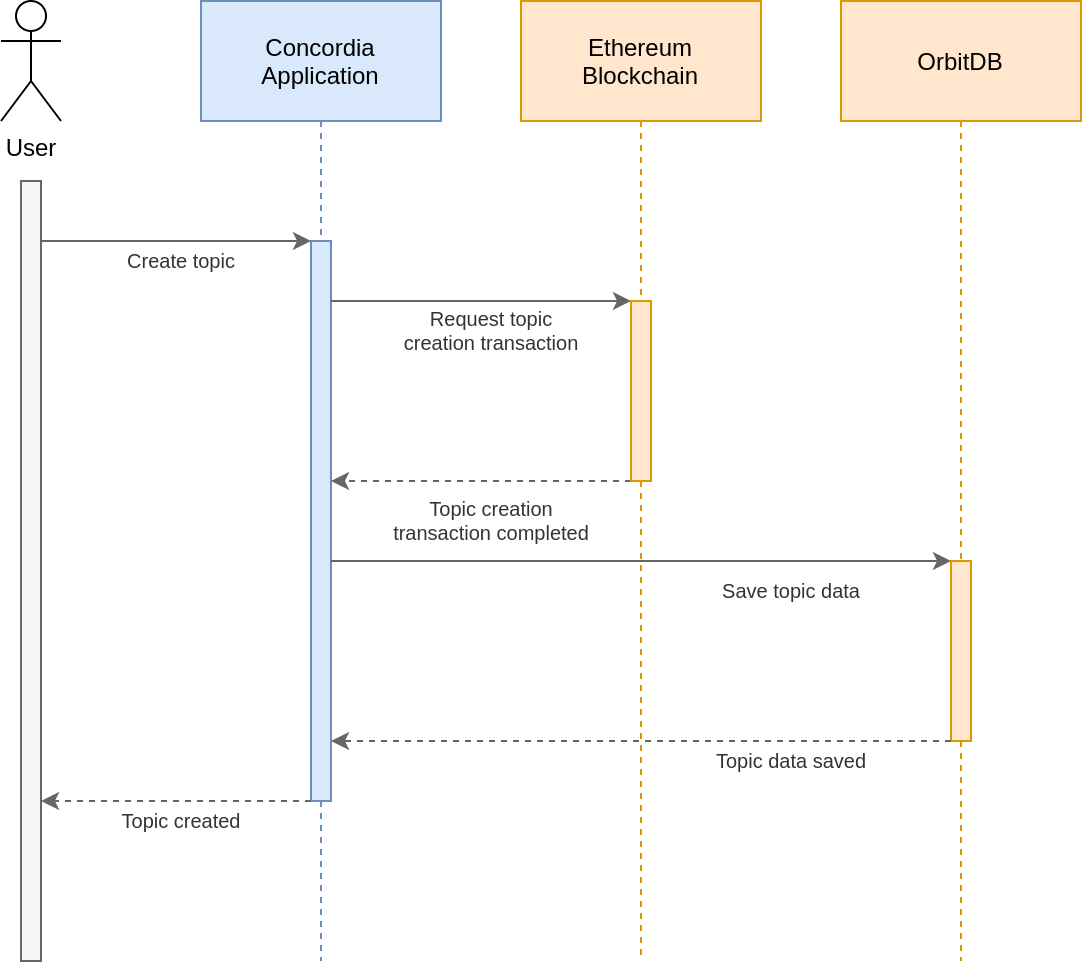
\includegraphics[width=.7\textwidth]{assets/figures/chapter-4/4.3.architecture-4.3.9.data-flow-insert.png}
    \caption{Διάγραμμα ακολουθίας δημιουργίας θέματος}
    \label{figure:4-3-data-flow-insert}
\end{figure}

Έστω, χρήστης που επιθυμεί να διαβάσει το προηγούμενο μήνυμα. Αρχικά, πρέπει να διαβαστεί ο πίνακας θεμάτων από το blockchain. Η πληροφορία αυτή εμπλουτίζεται από τα δεδομένα του κάθε θέματος, τα οποία ανακτώνται από τις προσωπικές βάσεις Orbit κάθε χρήστη. Έπειτα, εφόσον το θέμα βρεθεί και ο αύξων αριθμός του είναι γνωστός, πρέπει να διαβαστούν από το blockchain τα μεταδομένα των μηνυμάτων του θέματος και συγκεκριμένα η διευθύνσεις των δημιουργών τους. Τέλος, μέσω του IPFS πρέπει να γίνει αντιγραφή των προσωπικών βάσεων των δημιουργών του κάθε μηνύματος και να αναζητηθούν σε αυτές τα εκάστοτε μηνύματα. Στο σχήμα \ref{figure:4-3-data-flow-read} φαίνεται το διάγραμμα ροής της πληροφορίας κατά την ανάκτηση πληροφοριών από το σύστημα.

\begin{figure}[H]
    \centering
    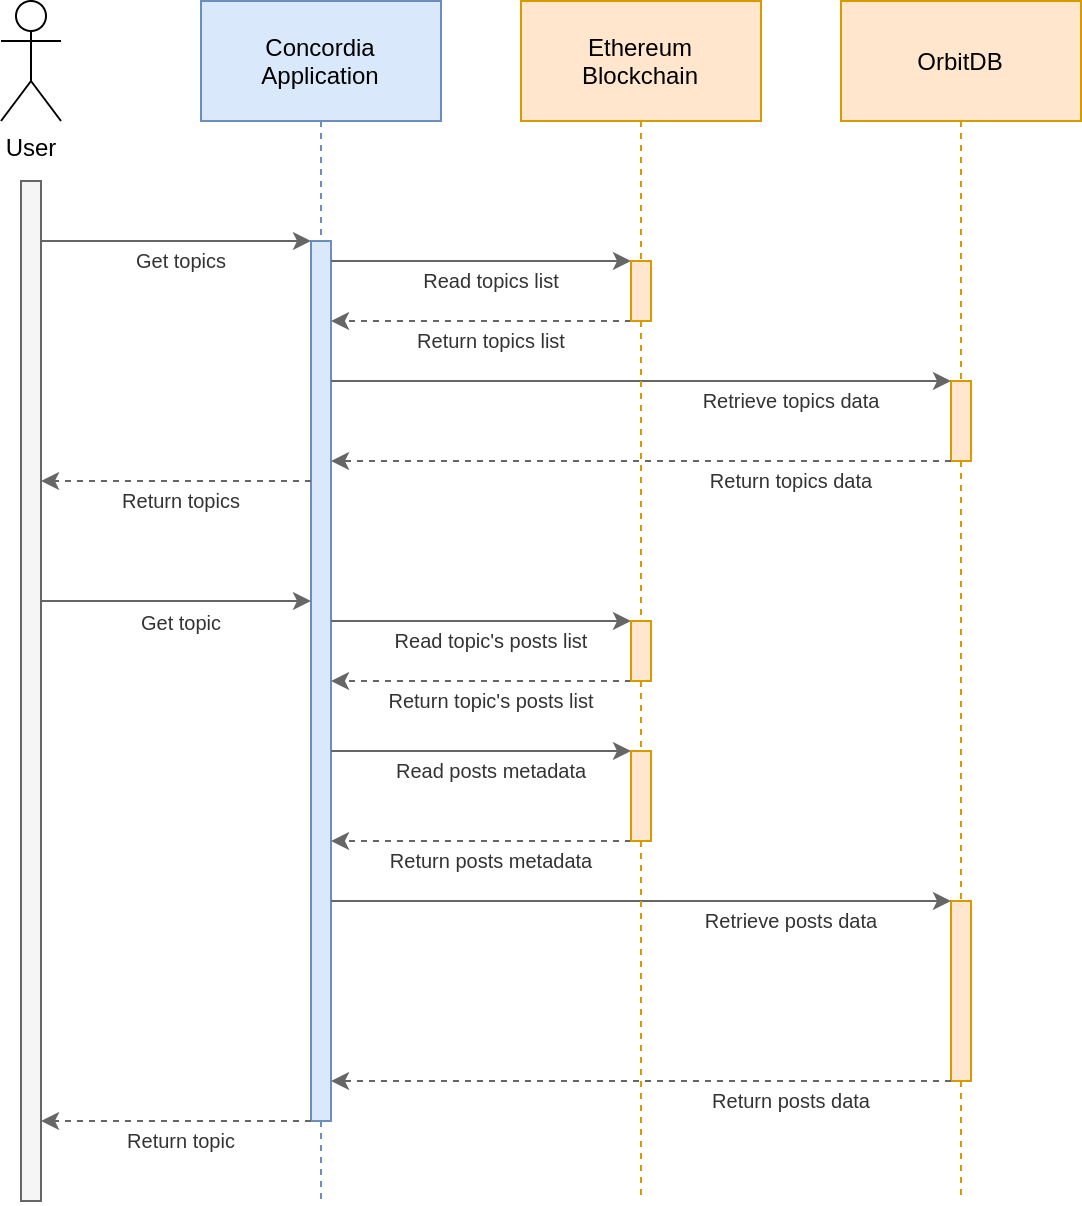
\includegraphics[width=.7\textwidth]{assets/figures/chapter-4/4.3.architecture-4.3.9.data-flow-read.png}
    \caption{Διάγραμμα ακολουθίας εύρεσης και ανάκτησης θέματος}
    \label{figure:4-3-data-flow-read}
\end{figure}
